\documentclass[14pt]{extbook}
\usepackage{multicol, enumerate, enumitem, hyperref, color, soul, setspace, parskip, fancyhdr} %General Packages
\usepackage{amssymb, amsthm, amsmath, latexsym, units, mathtools} %Math Packages
\everymath{\displaystyle} %All math in Display Style
% Packages with additional options
\usepackage[headsep=0.5cm,headheight=12pt, left=1 in,right= 1 in,top= 1 in,bottom= 1 in]{geometry}
\usepackage[usenames,dvipsnames]{xcolor}
\usepackage{dashrule}  % Package to use the command below to create lines between items
\newcommand{\litem}[1]{\item#1\hspace*{-1cm}\rule{\textwidth}{0.4pt}}
\pagestyle{fancy}
\lhead{Progress Quiz 6}
\chead{}
\rhead{Version C}
\lfoot{1430-1829}
\cfoot{}
\rfoot{test}
\begin{document}

\begin{enumerate}
\litem{
Determine the domain of the function below.\[ f(x) = \frac{6}{12x^{2} -32 x + 20} \]\begin{enumerate}[label=\Alph*.]
\item \( \text{All Real numbers.} \)
\item \( \text{All Real numbers except } x = a \text{ and } x = b, \text{ where } a \in [14.14, 15.28] \text{ and } b \in [15.67, 16.82] \)
\item \( \text{All Real numbers except } x = a, \text{ where } a \in [14.14, 15.28] \)
\item \( \text{All Real numbers except } x = a \text{ and } x = b, \text{ where } a \in [0.63, 1.58] \text{ and } b \in [1.16, 2.36] \)
\item \( \text{All Real numbers except } x = a, \text{ where } a \in [0.63, 1.58] \)

\end{enumerate} }
\litem{
Solve the rational equation below. Then, choose the interval(s) that the solution(s) belongs to.\[ \frac{48}{32x -72} + 1 = \frac{48}{32x -72} \]\begin{enumerate}[label=\Alph*.]
\item \( x_1 \in [0.25, 4.25] \text{ and } x_2 \in [0.25,3.25] \)
\item \( x \in [2.25,3.25] \)
\item \( x_1 \in [-2.25, -0.25] \text{ and } x_2 \in [0.25,3.25] \)
\item \( \text{All solutions lead to invalid or complex values in the equation.} \)
\item \( x \in [-2.25,-0.25] \)

\end{enumerate} }
\litem{
Solve the rational equation below. Then, choose the interval(s) that the solution(s) belongs to.\[ \frac{7x + 0}{4x + 5} + \frac{-7x^{2} +0 x + 0}{12x^{2} -x -20} = \frac{3}{3x -4} \]\begin{enumerate}[label=\Alph*.]
\item \( x \in [2.97,4.51] \)
\item \( x_1 \in [-0.36, -0.23] \text{ and } x_2 \in [-3.1,2.8] \)
\item \( x_1 \in [-0.36, -0.23] \text{ and } x_2 \in [2.2,4] \)
\item \( \text{All solutions lead to invalid or complex values in the equation.} \)
\item \( x \in [0.66,2.27] \)

\end{enumerate} }
\litem{
Determine the domain of the function below.\[ f(x) = \frac{3}{12x^{2} -6 x -18} \]\begin{enumerate}[label=\Alph*.]
\item \( \text{All Real numbers except } x = a \text{ and } x = b, \text{ where } a \in [-2, 0] \text{ and } b \in [-0.5, 2.5] \)
\item \( \text{All Real numbers except } x = a \text{ and } x = b, \text{ where } a \in [-11, -6] \text{ and } b \in [21, 27] \)
\item \( \text{All Real numbers except } x = a, \text{ where } a \in [-11, -6] \)
\item \( \text{All Real numbers except } x = a, \text{ where } a \in [-2, 0] \)
\item \( \text{All Real numbers.} \)

\end{enumerate} }
\litem{
Choose the equation of the function graphed below.
\begin{center}
    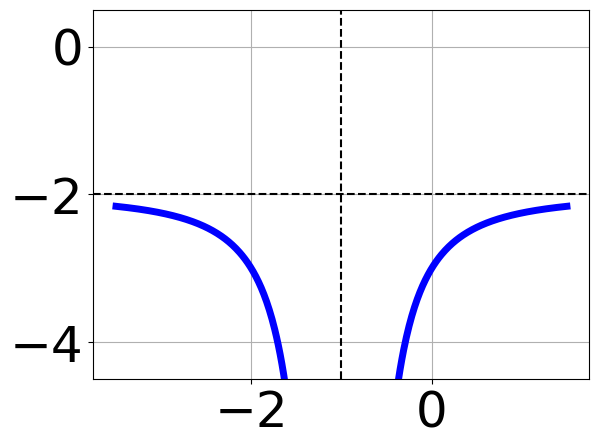
\includegraphics[width=0.5\textwidth]{../Figures/rationalGraphToEquationCopyC.png}
\end{center}
\begin{enumerate}[label=\Alph*.]
\item \( f(x) = \frac{1}{(x - 1)^2} + 1 \)
\item \( f(x) = \frac{-1}{x + 1} + 1 \)
\item \( f(x) = \frac{-1}{(x + 1)^2} + 1 \)
\item \( f(x) = \frac{1}{x - 1} + 1 \)
\item \( \text{None of the above} \)

\end{enumerate} }
\litem{
Choose the graph of the equation below.\[ f(x) = \frac{-1}{(x - 2)^2} + 3 \]\begin{enumerate}[label=\Alph*.]
\begin{multicols}{2}\item 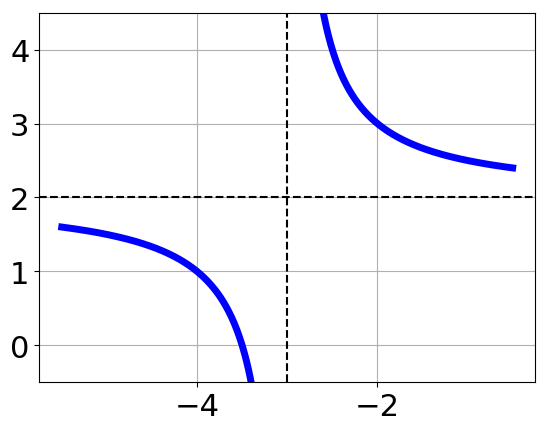
\includegraphics[width = 0.3\textwidth]{../Figures/rationalEquationToGraphAC.png}\item 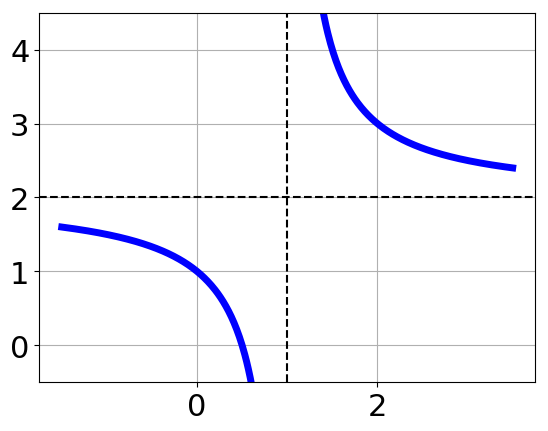
\includegraphics[width = 0.3\textwidth]{../Figures/rationalEquationToGraphBC.png}\item 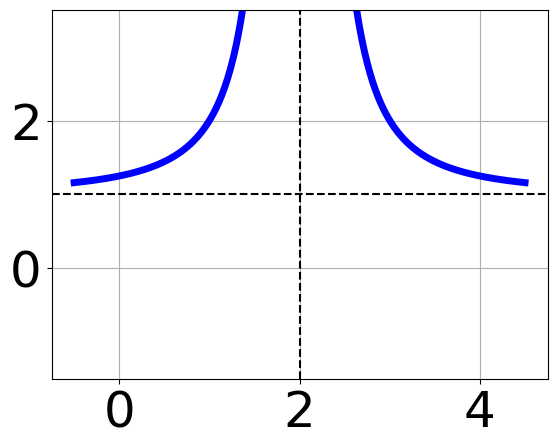
\includegraphics[width = 0.3\textwidth]{../Figures/rationalEquationToGraphCC.png}\item 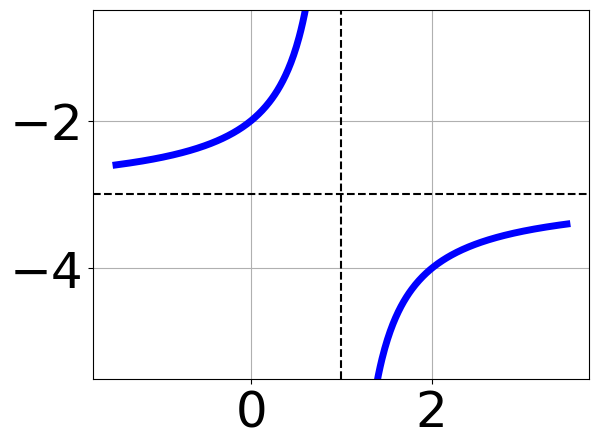
\includegraphics[width = 0.3\textwidth]{../Figures/rationalEquationToGraphDC.png}\end{multicols}\item None of the above.
\end{enumerate} }
\litem{
Solve the rational equation below. Then, choose the interval(s) that the solution(s) belongs to.\[ \frac{65}{52x + 39} + 1 = \frac{65}{52x + 39} \]\begin{enumerate}[label=\Alph*.]
\item \( \text{All solutions lead to invalid or complex values in the equation.} \)
\item \( x \in [-0.75,0.25] \)
\item \( x_1 \in [-0.75, 0.25] \text{ and } x_2 \in [-1.2,-0.1] \)
\item \( x \in [-0.25,1.75] \)
\item \( x_1 \in [-0.75, 0.25] \text{ and } x_2 \in [0.2,1.7] \)

\end{enumerate} }
\litem{
Choose the graph of the equation below.\[ f(x) = \frac{1}{x - 1} - 3 \]\begin{enumerate}[label=\Alph*.]
\begin{multicols}{2}\item 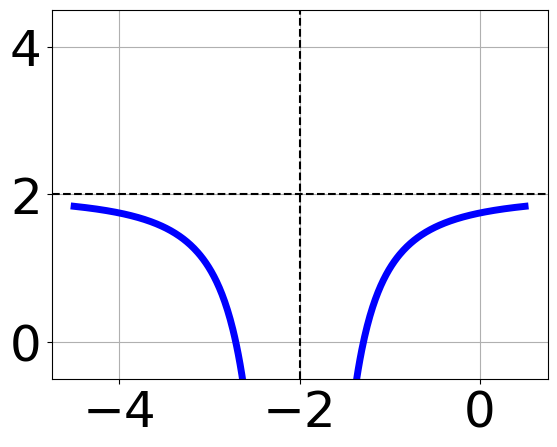
\includegraphics[width = 0.3\textwidth]{../Figures/rationalEquationToGraphCopyAC.png}\item 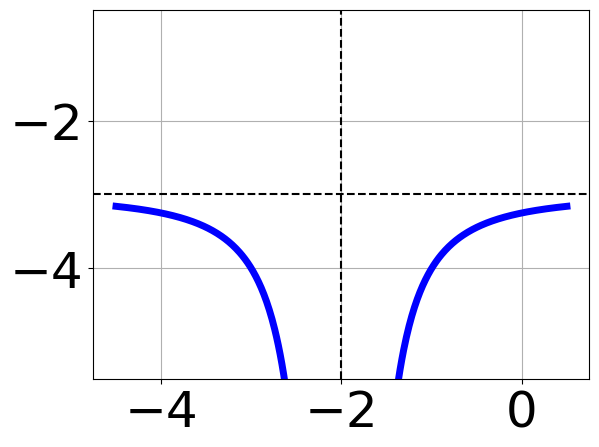
\includegraphics[width = 0.3\textwidth]{../Figures/rationalEquationToGraphCopyBC.png}\item 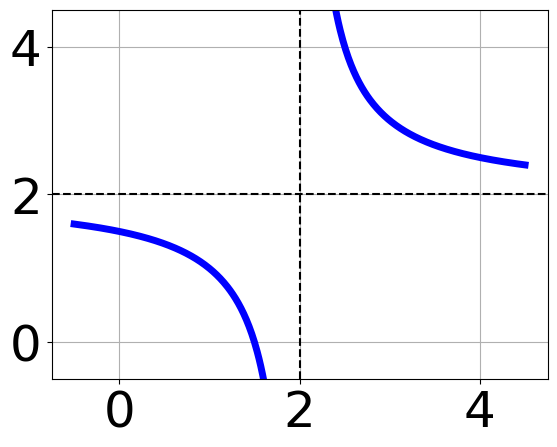
\includegraphics[width = 0.3\textwidth]{../Figures/rationalEquationToGraphCopyCC.png}\item 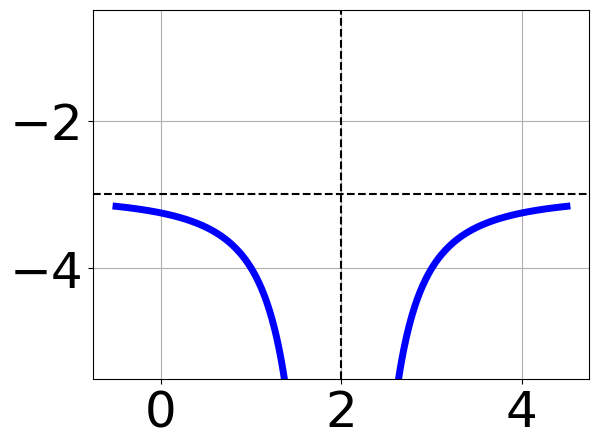
\includegraphics[width = 0.3\textwidth]{../Figures/rationalEquationToGraphCopyDC.png}\end{multicols}\item None of the above.
\end{enumerate} }
\litem{
Choose the equation of the function graphed below.
\begin{center}
    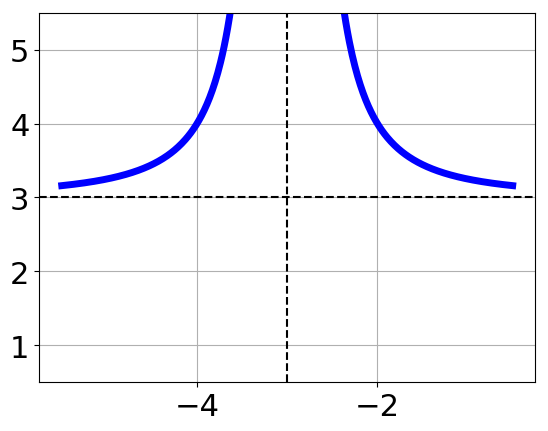
\includegraphics[width=0.5\textwidth]{../Figures/rationalGraphToEquationC.png}
\end{center}
\begin{enumerate}[label=\Alph*.]
\item \( f(x) = \frac{-1}{(x + 3)^2} + 2 \)
\item \( f(x) = \frac{1}{(x - 3)^2} + 2 \)
\item \( f(x) = \frac{-1}{x + 3} + 2 \)
\item \( f(x) = \frac{1}{x - 3} + 2 \)
\item \( \text{None of the above} \)

\end{enumerate} }
\litem{
Solve the rational equation below. Then, choose the interval(s) that the solution(s) belongs to.\[ \frac{7x + 0}{-7x -5} + \frac{-7x^{2} +0 x + 0}{-14x^{2} -45 x -25} = \frac{6}{2x + 5} \]\begin{enumerate}[label=\Alph*.]
\item \( \text{All solutions lead to invalid or complex values in the equation.} \)
\item \( x_1 \in [-11.4, -10] \text{ and } x_2 \in [-0.58,-0.22] \)
\item \( x_1 \in [-11.4, -10] \text{ and } x_2 \in [-0.98,-0.71] \)
\item \( x \in [-5.5,-1.1] \)
\item \( x \in [-0.9,0.2] \)

\end{enumerate} }
\end{enumerate}

\end{document}